\section{Ziel}
\label{sec:Ziel}
Ziel dieses Versuches ist es, den Zeeman-Effekt zu verifizieren. 
Dabei wird die Aufspaltung der roten und blauen Spektrallinie von Cadmium-Atomen untersucht, wenn
die Atome unter Einfluss eines Magnetfeldes stehen.

\section{Theorie}
\label{sec:Theorie}

%\begin{figure}
%  \centering
%  \includegraphics[width=0.55\textwidth]{Hysteresekurve.png}
%  \caption{Hysteresekurve [1].}
%  \label{fig:hkurve}
%\end{figure}

Der Zeeman-Effekt beschreibt das Phänomen, dass Spektrallinien von Atomen sich Aufspalten und eine 
gewisse Polarisation annehmen, wenn die Atome unter dem Einfluss eines Magnetfeldes stehen. 
Dieses Phänomen lässt sich nur quantenmechanisch beschreiben. 
Zunächst wird also die quantenmechanische Betrachtung eines Atoms erläutert.


\subsection{Quantenzahlen und magnetische Momente}

Bei einem Atom mit vielen Elektronen werden jedem Elektron andere Quantenzahlen zugeordnet. Nach dem 
Pauli-Prinzip können zwei Elektronen im selben Atom nicht exakt dieselben Quantenzahlen haben. 
Die Quantenzahlen beschreiben den Eigenspin des Elektrons durch die Spinquantenzahl $s$, den Bahndrehimpuls 
des Elektrons mit der Nebenquantenzahl $l$, den 
Gesamtdrehimpuls des Elektrons $j$, den Gesamtdrehimpuls der Elektronenhülle, also aller Elektronen $J$, 
den Kernspin $I$ und der Gesamtdrehimpuls des Atoms $F = I + J$. Im Folgenden werden aber nur Atome 
betrachtet, die einen Kernspin von Null haben, sodass der Gesamtdrehimpuls des Atoms gleich dem 
Gesamtdrehimpuls der Elektronenhülle $J$ ist.

Außerdem wird davon ausgegangen, dass die Elektronen in unterschiedlichen Schalen sitzen. Diese werden 
mit der Hauptquantenzahl $n$ beschrieben.
Die Elektronen besitzen auch magnetische Momente $\mu$. So gibt es noch die magnetische Quantenzahl 
des Bahndrehimpulses oder auch Orientierungsquantenzahl $m$ genannt.

%Bei Elektronen ist $s=\frac{1}{2}$, $l$ kann Werte zwischen Null und $n-1$ annehmen. 

Da die Elektronen geladen sind, und bewegte Ladung nach dem Biot-Savait-Gesetz ein B-Feld induzieren, 
sind die Drehimpulse und die magnetischen Momente miteinander verknüpft.


%Man betrachetet es so wie die Sonne und die Erde. Für das Elektron ist es so als würde der geladene Atomkern um ihn kreisen.
So gehört zu dem Bahndrehimpuls das magnetische Moment $\vec{\mu_l}$
\begin{equation*}
    \vec{\mu_l} = - \mu_B \sqrt{l(l+1)} \vec{l_e}
\end{equation*}
und zu dem Eigenspin das magnetische Moment $\vec{\mu_s}$
\begin{equation*}
    \vec{\mu_s} = - g_S \mu_B \sqrt{s(s+1)} \vec{s_e}.
\end{equation*}
Dabei ist $\mu_B = \frac{\hbar e}{2 m_e}$ das Bohrsche Magneton, $\vec{l_e}$ und $ \vec{s_e}$ sind die 
Einheitsvektoren in Richtung $\vec{l}$ bzw. $\vec{s}$
und $g_S$ ist der Landé-Faktor des Elektrons, er kann als ungefähr 2 angenommen werden. 
Der Proportionalitätsfaktor zwischen dem magnetischem Moment und dem Drehimpuls bzw. dem Spin wird 
gyromagnetischer Faktor genannt. Somit ist der 
Unterschied zwischen dem gyromagnetische Verhältnis von dem Elektronenspin und dem für den Drehimpuls
der Landé-Faktor des Elektrons $g_S \approx 2$.
Das gesamte magnetische Moment der Elektronenhülle $\vec{\mu}$ setzt sich aus allen magnetischen 
Momenten aller Elektronen in der Hülle zusammen. Allerdings nicht immer auf dieselbe Weise, da 
bei mehreren Elektronen die Drehimpulse und die magnetischen Momente miteinander wechselwirken
und es von den Atomeigenschaften abhängt in welcher Art und Weise. Dies wird im folgenden Näher erläutert. 



\subsection{Wechselwirklungsmöglichkeiten zwischen den Drehimpulsen und den magnetischen Momenten der Elektronen}

Die Wechselwirklungsmöglichkeiten zwischen den Drehimpulsen und den magnetischen Momenten der Elektronen 
sind sehr vielfältig. 
Vereinfacht werden hier nur zwei Grenzfälle betrachtet.

\subsubsection{jj-Kopplung}

Einmal werden schwere Atome betrachtet. Diese haben sehr viele Elektronen. Hier ist die Wechselwirkung 
zwischen Spin und Bahndrehimpuls eines Elektrons dominater als die Kopplung der verschiedenen Spins und 
Bahndrehimpulsen untereinander. So summieren sich zuerst die einzelnen Spins und Bahndrehimpulse zusammen 
zu einem Gesamtdrehimpuls der einzelnen Elektronen $j$ zu 
\begin{equation*}
    \vec{j_i} = \vec{l_i} + \vec{s_i}.
\end{equation*}
Die sich dann zu einem Gesamtdrehimpuls von der Elektronenhülle $J$ zusammentun:
\begin{equation*}
    \vec{J} = \sum{\vec{j_i}}.
\end{equation*}

\subsubsection{LS-Kopplung}

Bei Atomen kleinerer Ordnungszahl, ist die Wechselwirkung zwischen den einzelnen Spins und Bahndrehimpulsen 
dominant. Sie addieren sich erst zu einem Gesamtspin $S$
\begin{equation*}
    \vec{S} = \sum {\vec{s_i}}
\end{equation*}
und einem Gesamtbahndrehimpuls der Elektronenhülle $L$
\begin{equation*}
    \vec{L} = \sum {\vec{l_i}}
\end{equation*}
und dann zu dem Gesamtdrehimpuls der Elektronenhülle $J$
\begin{equation*}
    \vec{J} =  \vec{L} + \vec{S}.
\end{equation*}
Dabei sind nur die unabgeschlossenen Schalen wichtig, da sich die Impulse von abgeschlossenen Schalen 
gegenseitig aufheben.
Diese Art von Atom wird auch im folgendem Versuch näher untersucht. 


\subsection{Aufspaltung im Magnetfeld}

Aufgrund der Schalen hat ein Atom verschiedene Energienievaus.
Diese Spalten sich aber weiter auf. 
Durch den Elektronenspin kann auch ohne äußeres Magnetfeld, durch das durch den Elektronenspin 
bedingte magnetische Moment, eine Aufspaltung der Energienievaus erfolgen. Diese wird als Feinstruktur 
bezeichnet. 
%Wird der Kernspin miteinbezogen erfolgt eine weitere Aufspaltung zur Hyperfeinstruktur. 

Wird nun ein Atom einem äußeren Magnetfeld ausgesetzt, so richten sich die magnetischen Momente 
danach aus. Es erfolgt eine weitere Aufspaltung der Energienievaus der Elektronen, die Zeeman-Aufspaltung. 
Es gibt dann $2J+1$ Energienievaus.

Das gesamte magnetische Moment der 
Elektronenhülle $\vec{\mu}$ setzt sich zusammen aus 
\begin{equation*}
     \vec{\mu} =  \vec{\mu_L} + \vec{\mu_S}.
\end{equation*}
Das gesamte magnetische Moment der Elektronenhülle $\vec{\mu}$ und der Gesamtdrehimpuls der 
Elektronenhülle $\vec{J}$ zeigen dabei nicht in dieselbe Richtung, siehe Abblildung \ref{fig:mm}.

\begin{figure}
  \centering
  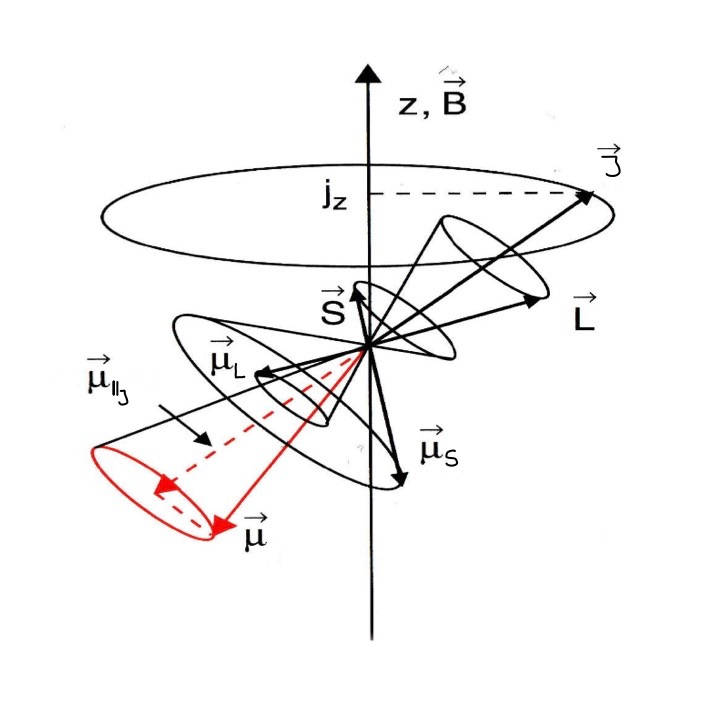
\includegraphics[width=0.55\textwidth]{mag.mo.jpeg}
  \caption{Drehimpulse und magnetische Momente [5](mit geänderten Indizes und Bezeichnungen).}
  \label{fig:mm}
\end{figure}
\FloatBarrier

Das gesamte magnetische Moment der Elektronenhülle präzesiert aber um die zum Gesamtdrehimpuls parallele 
Komponente des gesamten magnetischen Moments $\vec{\mu}_{\symup{ll_J}}$. Sodass der Erwartungswert nur 
$\vec{\mu}_{\symup{ll_J}}$ ergibt. Der Betrag von dem gesamten magnetischen Moment ergibt sich durch 
\begin{equation*}
    \lvert \vec{\mu} \rvert = \mu_B \sqrt{J (J+1)} \frac{3J(J+1)+ S(S + 1) - L (L+1)}{2 J(J +1)} = \mu_B \sqrt{J (J+1)} g_J.
\end{equation*}
Der Faktor 
\begin{equation}
    g_J = \frac{3J(J+1)+ S(S + 1) - L (L+1)}{2 J(J +1)},
    \label{eqn:gJ}
\end{equation}
wird als Landé-Faktor bereichnet. 

Die verschiedenen Energienievaus ergeben sich dann aus der Richtungsquantelung. Zwischen dem Magnetfeld $B$ 
und dem gesamten magnetischen Moment $\vec{\mu}$ sind nur ganzzahlige Vielfache von $g_J \mu_B$ erlaubt:
\begin{equation*}
    E_{\symup{zu}} = m g_J \mu_B B,
\end{equation*}
wobei $E_{\symup{zu}}$ die zusätzliche Energie ist, die das gesamte magnetische Moment unter Einfluss 
eines äußeren Magentfeldes bekommt. Die Orientierungsquantenzahl $m$ kann nur die ganzzahligen 
Werte von $J$ bis $-J$ annehmen. Das sind genau $2J+1$ verschiedene Werte, also $2J+1$ verschiedene 
Energienievaus.
Die zusätzliche Energie $E_{\symup{zu}}$ ergibt auch den Abstand zwischen den Energienievaus. Bei stärkerem 
Magnetfeld driften die Energienievaus weiter auseinander. Der Paschen-Back-Effekt beschreibt dabei das 
Phänomen, dass die Spin- und Bahndrehimpulse bei sehr hohen Magnetfeldern entkoppeln.
%-> keine Zeeman-Aufspaltung 

Aus Übergängen zwichen diesen Energienievaus entsteht auch die Aufspaltung der Spektrallinien bei 
Atomen im äußeren Magnetfeld. Es sind aber nur bestimmte optische Übergänge erlaubt, was mit den 
Auswahlregeln beschrieben wird. 


\subsection{Die optischen Übergänge}

%kommen aus Schrödinger-Gleichung
Übergänge können nur stattfinden, wenn die Auswahlregeln erfült sind. Dabei gilt: 
Die Differenz der Orientierungsquantenzahl $m$ der beiden Energienievaus muss $\symup{\Delta}m = \pm 1 \vee 0$ 
betragen. Dabei ist Licht, dass durch einen Übergang mit $\symup{\Delta}m=0$ entsteht ein $\pi$-Übergang 
und linear polarisiert. %um das magnetfeld 
Ist $\symup{\Delta}m = 1$ wird der Übergang als $\sigma_{+}$ bezeichnet und rechts 
zirkular polarisiert. Bei $\symup{\Delta}m = -1$ entsteht ein links zirkular polarisierter $\sigma_{-}$-Übergang.

Im diesem Versuch wird die rote und die blaue Spektrallinie einer Cd-Lampe betrachtet. 
Die Aufspaltung der Spektrallinie der roten wird dabei durch den normalen Zeeman-Effekt hervorgerufen, 
die Aufspaltung der blauen durch den annormalen. 

\subsubsection{Der normale Zeeman-Effekt}

Der normale Zeeman-Effekt tritt dann auf, wenn für den Spin gilt: $s=0$. Dann ergibt sich der 
Landé-Faktor $g_J$ mit Formel \ref{eqn:gJ} und immer zu 1. 
Der Energie $E$ der Spektrallinien berechent sich durch
\begin{equation}
    E = (m_i g_{Ji} - m_j g_{Jj}) \mu_B B + E_0.
    \label{eqn:E}
\end{equation}
Da alle Landé-Faktoren gleich 1 sind, sind immer drei Spekrallinien möglich, 
für jeweils einen $\pi$- oder $\sigma_{\pm}$-Übergang:
\begin{align*}
    \symup{\Delta}m = 0 &: \symup{\Delta}E = 0 \\
    \symup{\Delta}m = -1 &: \symup{\Delta}E =\mu_B B\\
    \symup{\Delta}m  = 1 &: \symup{\Delta}E =- \mu_B B,
\end{align*}
und das unabhänging von den Quantenzahlen.
%Benachbarte Energienievaus haben dabei immer dieselben Energienievaus-Abstände.

In Abblildung \ref{fig:rot} ist das Termschema für die rote Linie der Cd-Lampe mit dem normalen 
Zeeman-Effekt zu sehen. Auf der linken 
Seite ohne Magnetfeld, auf der rechten Seite mit. 

\begin{figure}
  \centering
  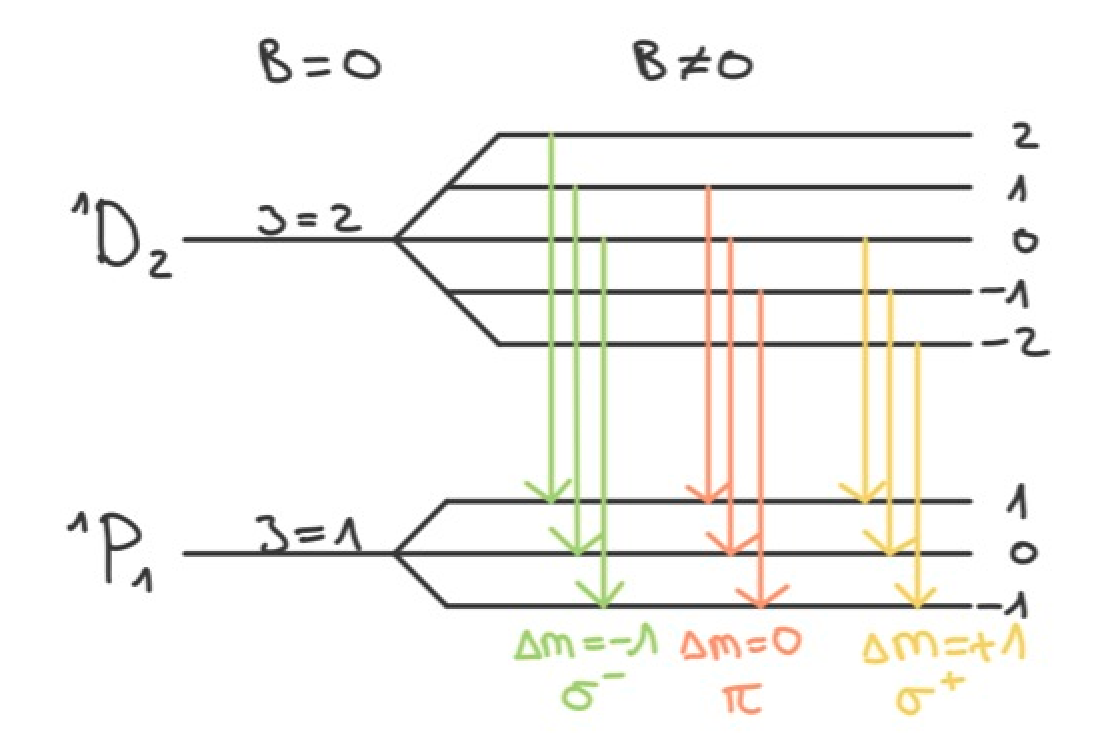
\includegraphics[width=0.75\textwidth]{rot2.png}
  \caption{Termschema der roten Linie der Cd-Lampe.}
  \label{fig:rot}
\end{figure}

%Will man die Spekrallinien aufnehmen, ist zu Berücksichtigen das die Polarisation des Lichtes 
%entlang des Magentfeldes erfolgt. So erscheinen die zirkular polarisierte Übergänge linear wenn 
%die Übergänge senktrecht zum Magnetfeld beobachtet werden. Die linearen Übergänge können nur aus senkrechter 
%Richtung und aus longitudinaler gar nicht beobachtet werden. 
%In diesem Versuch werden die Linien aus transversaler, also senkrechter Richtung betrachtet. Es können 
%also alle drei Übergänge beobachtet werden erscheinen linear polarisiert.
%Oder nur 2?




\subsubsection{Der annormale Zeeman-Effekt}

Bei annormalen Zeeman-Effekt ist der Spin ungleich Null. Dieser Fall ist der häufigere.
Hier sind die Landé-Faktoren der unterschiedlichen Energienievaus nicht mehr gleich, da der Spin nicht mehr Null ist. 
Es sind also nicht mehr immer nur drei Spektrallinien, da die Energiedifferenz zwischen den 
Spekrallinien nun von den Quantenzahlen abhängt (vgl. Formel \ref{eqn:E}). 

In Abblildung \ref{fig:blau} ist das Termsch$\sigma_{+}$ema für die blaue Linie der Cd-Lampe mit dem annormalen 
Zeeman-Effekt zu sehen. Hier sind Spekrallinien der Energien $\symup{\Delta}E = \pm 2 \mu_B B, \pm \frac{3}{2} \mu_B B, \pm \frac{3}{2} \mu_B B$ 
oder $0$ möglich. Diese Energiedifferenzen sind auch in der Abblildung eingezeichnet.

\begin{figure}
  \centering
  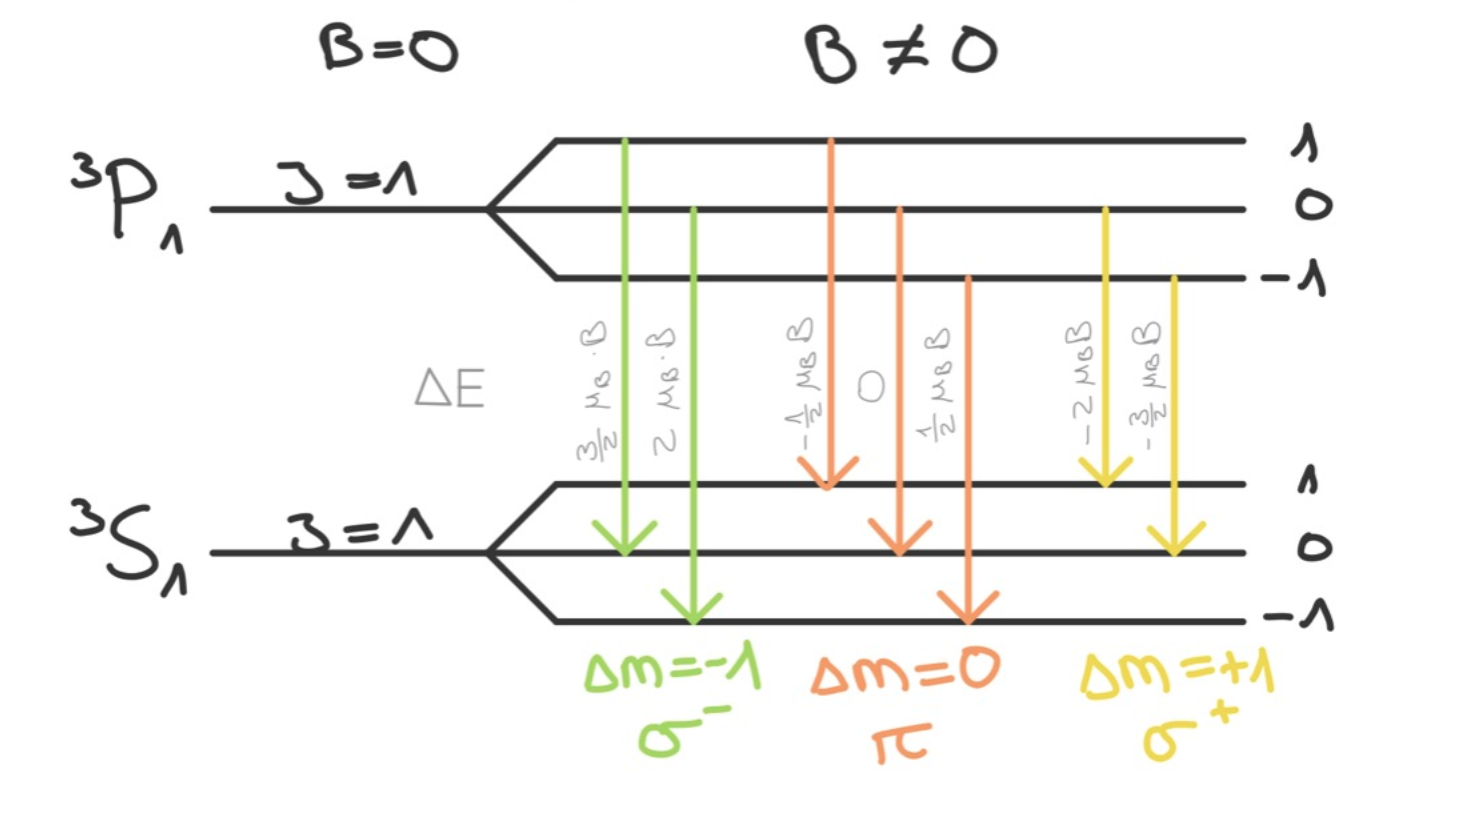
\includegraphics[width=0.75\textwidth]{blau2.png}
  \caption{Termschema der blauen Linie der Cd-Lampe.}
  \label{fig:rot}
\end{figure}
\FloatBarrier

%Auch hier werden die Spekrallinien transversal beobachtet, dass nur die $\sigma$-Übergänge sichtbar sind.
%Von den sieben Spekrallinien werden also nur vier beobachtet.
